\chapter{Obtención de características}

\section{Descripción de las propiedades de los objetos del ámbito}

Haciendo notar que nuestra base de datos se centra en los deportes, no es de extrañar que aparezca una gran cantidad de propiedades sobre estos. Estas las hemos clasificado, teniendo en cuenta su naturaleza, en \emph{categorías}, \emph{instalaciones}, \emph{accesorios}, \emph{jugadores} y \emph{otros}. Dando como resultado las siguientes caracterísitcas posibles para cada deporte y los valores que pueden tomar cada una de ellas: 

\begin{itemize}
\item categorías:
	\begin{itemize}
	\item acuático
	\item nieve
	\item equipo
	\item raqueta
	\item precisión
	\item motor
	\item atletismo
	\item combate
	\end{itemize}
	
\item instalaciones:
	\begin{itemize}
	\item campo césped
	\item campo tierra
	\item pista hielo
	\item pista césped
	\item pista tierra
	\item pista dura
	\item cancha parqué
	\item pista cemento
	\item pista césped sintético
	\item pista moqueta
	\item pista atletismo
	\item red
	\item canasta
	\item portería
	\item trampolín
	\item piscina
	\item valla
	\item circuito
	\item tatami
	\item ring
	\end{itemize}
	
\item accesorios:
	\begin{itemize}
	\item cuerda
	\item pesas
	\item bate
	\item casco
	\item raqueta
	\item pala
	\item balón
	\item pelota
	\item patín
	\item monopatín
	\item tabla
	\item vela
	\item cometa
	\item caña pescar
	\item paracaídas
	\item parapente
	\item ala delta
	\item snowboard
	\item esquí
	\item palo golf
	\item guantes
	\item kimono
	\item cinturón
	\item gafas natación
	\item gafas buzo
	\item tubo buzo
	\item bombona
	\item aletas
	\item piragüa
	\item kayak
	\item jabalina
	\item disco
	\item pértiga
	\item martillo
	\item bola
	\item tablero
	\item ficha
	\item taco
	\item bumerán
	\item frisbee
	\item dardo
	\item diana
	\item bicicleta
	\item sable
	\item espada
	\item florete
	\item stick
	\item bolo
	\item cepillo
	\item pistola
	\item rifle
	\item aro
	\item maza
	\item cinta
	\item step
	\end{itemize}

\item jugadores: \emph{Número de jugadores que compone un equipo (1 si el deporte es individual).}

\item otros:
	\begin{itemize}
	\item caballo
	\item barco
	\item coche
	\item moto
	\item avión
	\item globo
	\end{itemize}
\end{itemize}
% 
% 
% 
% \section{Descripción de las relaciones entre los objetos del ámbito y las propiedades}
% 
% Teniendo en cuenta las propiedades nombradas anteriormente, la relación entre ellas y entre los objetos del ámbito puede verse reflejada en el siguiente diagrama:
% 
% \begin{figure} [ht]
% \begin {center}
% 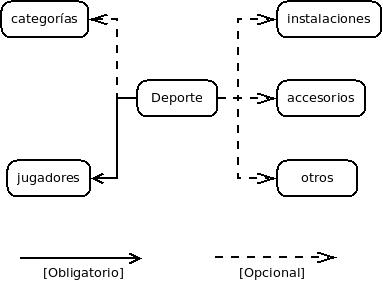
\includegraphics[scale = 0.6]{./Deportes.jpeg}
% \caption{Diagrama de relación entre objetos y propiedades}
% \end {center}
% \end{figure}
% 
% Como se observa en el esquema anterior, cada deporte debe de tener asigando, al menos, una categoría y un número de jugadores por equipo. El resto de campos (intalaciones, accesorios y otros), son opcionales, ya que existen deportes que no tenga alguno de ellos, aunque sí sería obligatorio poseer los atributos de estos campos en el caso que el deporte tuviese algún tipo de instalación, accesorio u otro complemento; es decir, la no obligatoriedad del campo hace flexible reflejar todos los deportes de la base de datos, pero siempre que un deporte posea una de esas propiedades tendrá que constar obligatoriamente.
% 
% 
